\documentclass{article}

\usepackage{fullpage}
\usepackage{graphicx}
\usepackage{clrscode}
\usepackage{amsmath}

\title{CS787 Homework 5}
\author{Mikola Lysenko}

\begin{document}

\maketitle{}

\paragraph{} \textbf{1.}
\begin{itemize}
\item{i.} By the definition of $G_f$, the capacities $c_f(u,v) = c(u,v) - f(u,v)$.  If $f'$ is a flow on $G_f$ we have
\begin{eqnarray*}
f'(u,v) & \leq & c(u,v) - f(u,v) \\
f'(u,v) + f(u,v) & \leq & c(u,v)
\end{eqnarray*}
So, $f' + f$ obeys capacity constraints on $G$.  Skew symmetry and flow conservation are trivially satisfied, and so $f+f'$ is a flow in $G$.  The opposite direction follows a symmetric argument, reversing the order of the two equations above.

\item{ii.}
We start with the forward direction.  Let $f'$ be a max flow on $G_f$.  Suppose that $|f + f'|$ is not maximal, and so there exists some augmenting path on $f + f'$ within $G$.  This path must be a flow on $G_f$, and moreover it must augment $f'$ by part i.  However, this is a contradiction since $f'$ is maximal, and so $f + f'$ must be maximal.

Now let $f + f'$ be maximal in $G$ and suppose $f'$ has some augmenting path in $G_f$.  Then by the part i again, this path also augments $f + f'$ and so $f + f'$ is not maximal.  Once again, this is a contradiction and so $f'$ is maximal in $G_f$.

\item{iii.}
\[ |f + f'| = \sum \limits_{v \in V} f(s, v) + f'(s, v) = \sum \limits_{v \in V} f(s, v) + \sum \limits_{v \in V} f'(s,v) = |f| + |f'| \]
\end{itemize}

\paragraph{} \textbf{2.}
Given a vertex disjoint path, $p = v_1, v_2, ... v_n$ in $G$, the capacity of the path is defined as $|p| = \min \limits_{i \in [n-1]} c(v_i, v_i+1)$, which is associative and monotone on $v_i$.  Therefore, Dijkstra's algorithm will find the maximum capacity path from $s$ to $t$ in worst case $O( |E| + |V| \log{ |V| } )$ (by previous homework).  The arguments from problems 3-4 show that the number of iterations is bounded by $O(|E| \log{M})$, so the running time of this flow algorithm is bounded by $O(|E| \log{M} (|E| + |V| \log{|V|}))$.  

\paragraph{} \textbf{3.}
Given the flow $f$ and network $G$, construct the residual flow network $G_{f'}$ such that $f'$ is a max flow in the residual $G_f$.  From problem 1, we know the following:
\begin{itemize}
\item{i.} Any flow on $G_{f'}$ is also a flow on $G$.
\item{ii.} $f$ must be a max flow in $G_{f'}$
\item{iii.} For any flow, $p$, on $G_{f'}$; $|f - p| = |f| - |p|$
\end{itemize}
If the capacity of $f$ is 0, then we are done.  Otherwise, the max-flow/min-cut theorem assures the existence of some path flow, $p$, on $G_{f'}$ with $|p| > 0$, so take $p$ to be a path flow maximum capacity and augment $G_{f'}$ by $p$ to obtain the residual $G_{f' + p}$.  By the above items, there exists a max flow $f''$ on $G_{f' + p}$ such that $f'' = f + p$, and since the capacity $G_{f'+p} < G_{f'}$ and all flows are integer valued, this sequence eventually reaches 0 and thus each flow can be written as the sum of some number of saturated path flows, $p_1, p_2, ... $ plus some 0 flow and ordered such that $|p_i| \geq |p_{i+1}|$.\footnote{This much was shown in class.}

Now suppose that when we are all done we have more than $|E|$ path flows; then at least two paths must saturate the same edge.  Take the largest capacity path flow, $p_1$ and check it's blocking edges against all remaining flows.  If at least one edge is contained in no other flow, then remove $p_1$ and that edge and augment $f$ by $p_1$.  Otherwise, there is some path flow $p'$ such that $|p'| \leq |p_1|$ which shares some edge $u,v$ and looks like one of the following two cases:

\begin{center}
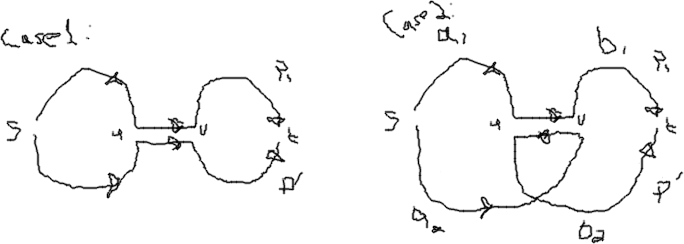
\includegraphics[height=1.5in]{5-3-1.png}
\end{center}

In case 2, we adjust all capacities in $p_1$ to $|p_1| - |p'|$, add the path flows $a_1 . b_2$, $a_2 . b_1$ with capacity $|p'|$ and remove $p_2$.  This construction does not change the total path capacity, and both $a_1 . b_2$ and $a_2 . b_1$ are valid flows, since the capacity from $s$ to $u$ (sym. $v$ to $t$) is greater than $|p_1| = |p'| + |p_1 - p'|$.  Repeat this for each path which is incident to this edge and traveling in the opposite direction.  Afterwords all flows must be traveling in the same direction along this edge, thus reducing the problem to case 1.

In case 1, take all flows incident to blocking edges of $p_1$ and transfer as much capacity as possible to $p_1$.  One of two situations will happen:
\begin{itemize}
\item{a.} Some edge in $p_1$ will block in which case we repeat 
\item{b.} One of the augmenting flows will run out of capacity. 
\end{itemize}
In the situation a, we must eventually run into some edge which is can not be augmented by any other path flows and thus can not be shared by any path - at which point we may augment the remaining $f$ by $p_1$ and remove its new blocking edge from $G$ as described above.  In situation b, we decrease the total number of paths without decreasing the total number of edges, thus decreasing the total number of paths.  At the end of this process, $f$ was augmented no more than $O(|E|)$ times, thus we have shown by construction that $f$ can be written as a sum of no more than $O(|E|)$ path flows, proving the theorem.

\paragraph{} \textbf{4.} (continuing from the midpoint of 3)
For each maximum augmenting path, $p$, from above we know that there are at most $|E|$ edges in $G_{f'}$ and that $|p| = c(u,v) \geq \frac{ |G_{f'}| } { |E| }$, for some $u,v \in V$.  Therefore, the augmented graph, call it $G_1$, has capacity
\[ |G_1| \leq (1 - \frac{1}{|E|})|G_{f'}| \]
This argument\footnote{Also done in class.} applies for each path, $p_i$, giving the general recurrence:
\[ |G_{i+1}| \leq (1 - \frac{1}{|E|})|G_i| \]
Which expands into:
\[ |G_{i+1}| \leq (1 - \frac{1}{|E|})^i |f| \]
Because all flows are integer capacities, at some point the quantity $G_i$ reaches 1, then 0.  To solve for this point, we wish to find a value for $i$ such that:
\[ (1 - \frac{1}{|E|})^i |f| = 1 \]
Which gives:
\[ i = \log_{\frac{ |E| - 1 }{ |E| }} (\frac{1}{|f|}) = \frac{ -\log{|f|} }{ \log{(|E| - 1)} - \log{|E|} } \]
For sufficiently large values of $|E|$, $\log{(|E| - 1)} - \log{|E|}$ approximates the derivative of $-\log{|E|}$, which is $-1/|E|$, and so we conclude that the sequence terminates in at most $O(|E| \log{|f|})$.

\paragraph{} \textbf{5.}
Let $p$ be the shortest augmenting path from the hypothesis and construct $G_p$ by augmenting via $p$.  Pick some vertex $u$ in $G, G_p$ and suppose that the distance from $u$ to the source in $G_p$ is larger than that of $G$.  If this was true, then along a shortest path from $s$ to $u$ in $G_p$, there must be some vertex $v$ directly before $u$ which added some new edge from $v$ to $u$ on $p$.  However, this would mean that $u$ came before $v$ in $p$ and so the distance from $u$ to $s$ should be one less than the distance from $v$ to $s$.  Therefore, we have a contradiction and the distance from any vertex to the source must be increasing, and so the length of any augmenting path must also be increasing.

\paragraph{} \textbf{6.}
Continuing on the above argument, pick the saturated edge $(u,v)$ of some augmenting path with $u$ occurring before $v$.  Next time this edge is selected, it must be augmented from $v$ to $u$ so the distance of $u$ to the source must have increased by 1.  Since each path augments one edge, and the maximum distance to the source for any vertex is $|V|$, the total number of paths is bounded above by $O(|V| |E|)$.

\paragraph{} \textbf{7.}
Let $G$ be a bipartite graph with vertex set $V = A \cup B$ partitioned by $A,B$ such that $E = \{ (u, v) | u \in A, v \in B \}$.  Construct a source $s$ and add edges $\{ (s,a) | a \in A \}$ and sink $t$ with additional edges $\{ (b, t) | b \in B \}$ and set all capacities to 1.  For any flow on $G$, the degree from any vertex in $A$ to $B$ is at most 1, and symmetrically for the degree of any vertex in $B$, so the flow must be a matching.  Moreover, for any matching from $A$, $B$, we may also construct a flow by augmenting the paths from $s-A-B-t$ trivially.  Since the capacity of the flow is the same as the the number of edges between $A,B$, a maximum flow yields a maximum matching.

\paragraph{} \textbf{8.}
First, observe that the minimum subset of the graph for disconnection only contains edges because if we were to delete a vertex and its surrounding edges, we could have also disconnected the graph by deleting only its edges.  Next assume without loss of generality that $G$ is connected, otherwise nothing need be removed at all.  Now consider the problem of determining the fewest number of edges to disconnect some vertex $u$ and another vertex $v$.  To do this, we can compute the maximum flow from $u$ to $v$ on $G$ with unit capacity edges and apply Menger's theorem.  By the max-flow/min-cut theorem, a cut in this graph would be a minimal collection of edges splitting $u,v$ into separate connected components (capacity from $u \rightarrow v = 0$ $\implies$ no paths from $u \rightarrow v$).  Repeating this for each distinct pair of vertices and taking the cut with minimum cardinality gives the minimum size subset for disconnecting $G$.

\end{document}
